\section{Exploring Interleaving Space}
\label{s:design}


In this section, we describe our approach to effectively explore the
search space of thread interleaving.
%
We first describe the key idea of our
approach~(\autoref{ss:overview}). Then, we illustrate our coverage
metric in the concurrency dimension~(\autoref{ss:coverage}), and the
instruction scheduling algorithm to quickly saturate the
coverage~(\autoref{ss:scheduler}).



While this section focuses only on exploring the search space of
thread interleaivng of given threads, \autoref{s:impl} describes the
whole design of \sys for expanding both code coverage and interleaving
coverage.


\subsection{Key Idea: Segmentizing thread interleaving}
\label{ss:overview}

% Overall 1 2 3 4 5
% 74 0 22 33 12 7

Our key idea starts from an extensive survey conducted by Shan Lu
\etal~\cite{learningfrommistakes}.
%
According to the survey, 92.4\% (97 out of 105) of concurrency bugs
they study manifest if a partial order of at most four memory accesses
are enforced;
%
Specifically, out of 105 concurrency bugs, 7 depend on one memory
access~\footnote{this case can happen only for deadlock bugs that a
  thread waits for a lock already acquired by itself.}, 25 depend on
two memory accesses, 53 depend on three memory accesses, and 12 depend
on four memory accesses.
%
The example described in \autoref{fig:cve-2019-6974} also follows this
survey since the uninitialized access is triggered depending on the
execution order of three memory accesses.


This survey suggests a balance point of a trade-off between the
completeness of the bug-finding functionality and the complexity of
exploring the search space of thread interleaving;
%
If one searches for all interleaving instances, he or she is able to
discover all concurrency bugs with a cost of astronomical time, and
if one focuses on the execution order of at most two instructions, he
or she quickly gets his job done with a risk of a high chance of
missing many (\eg, about 70\%) concurrency bugs.
%
Whereas, this paper sits between these two extremes. We track and
search for execution orders of at most four memory accesses to make
the problem tractable while maintaining a strong bug-finding
capability.



\PP{Segmentizing thread interleaving}
%
\begin{figure}[t]
  \subfloat[Interleaving instance]{
    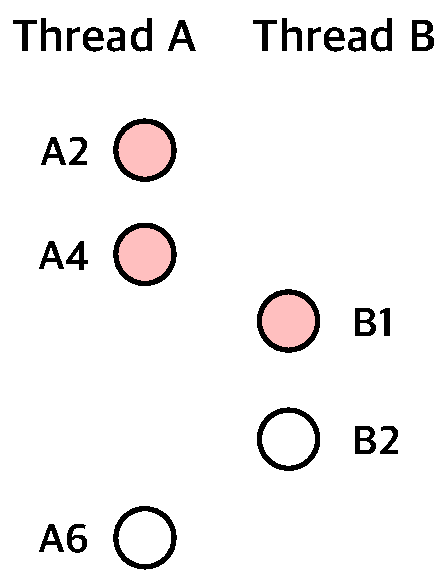
\includegraphics[width=0.35\linewidth]{fig/intuition-a.pdf}
  }
  \hfill
  \subfloat[Interleaving segments]{
    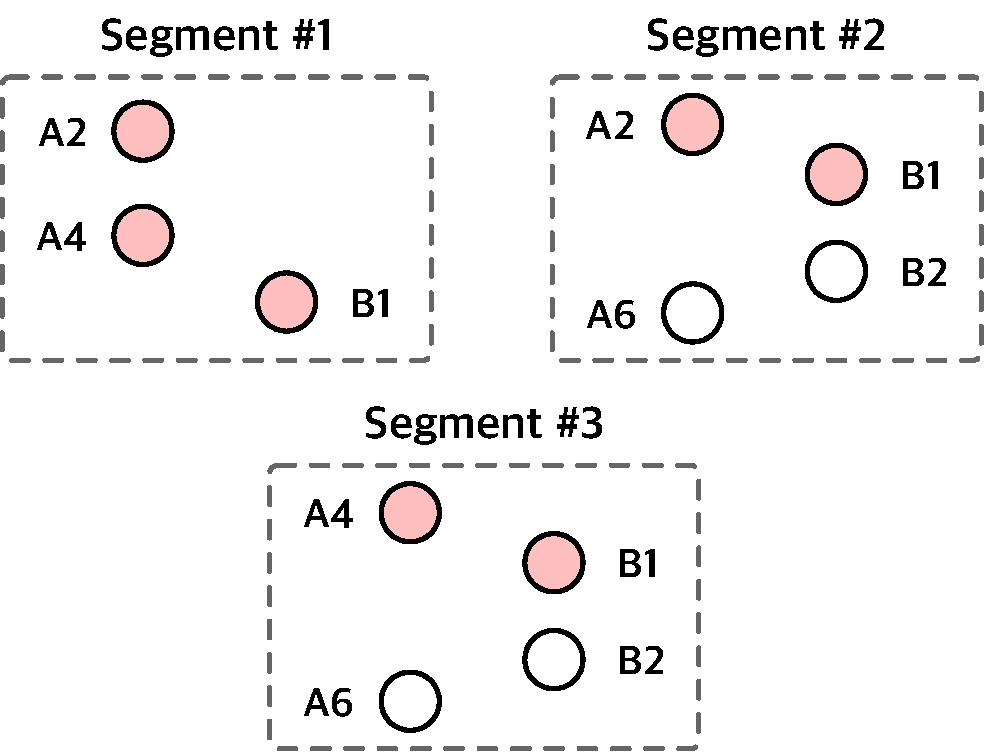
\includegraphics[width=0.55\linewidth]{fig/intuition-b.pdf}
  }
  \caption{}
  \label{fig:keyidea}
\end{figure}
%
Based on the survey, The key idea of our approach is to consider an
instance of thread interleaving as \textit{a composition of
  interleaving segments}, where each interleaving segment represents
the execution order of a small number of memory accesses.
%
In particular, after executing threads concurrently, we firstly model
an execution of these threads as a totally-ordered instruction
sequence.
%
And then, we group a small number of instructions (\eg, four
instructions) as a segment to track which segments are contained in
the execution and to search for unobserved segments in future
iterations.


\autoref{fig:keyidea} visualizes our key idea.
%
Let us assume we execute the two system calls in
\autoref{fig:cve-2019-6974}, and while executing the two system calls,
we track memory access operations conducted by the two system calls
with timestamps.
%
With traced memory access operations, we construct a totally-ordered
instruction sequence as described in \autoref{fig:keyidea}-(a).

we can decompose the interleaving instance into three interleaving
segments as described in \autoref{fig:keyidea}-(b).


It is worth noting that instructions in a segment \dr{}

can be overlapped; in this example,
\texttt{Segment \#1} and \texttt{Segment \#2} are overlapped over XXX.





\PP{Benefits of thread interleaving segmentization}
%
This approach provides two remarkable benefits.
%
\textbf{i)} Tracking interleaving segments is a befitting choice to
determine if any \textit{interesting} thread interleaving remains.
%
As mentioned above, most concurrency bugs manifest depending on the
execution order of four memory accesses.
%
In this perspective, whether or not an interleaving instance causes a
concurrency bug depends on whether a problematic segment is contained
in the instance of thread interleaving.
%
\dr{}



\begin{figure}[t]
  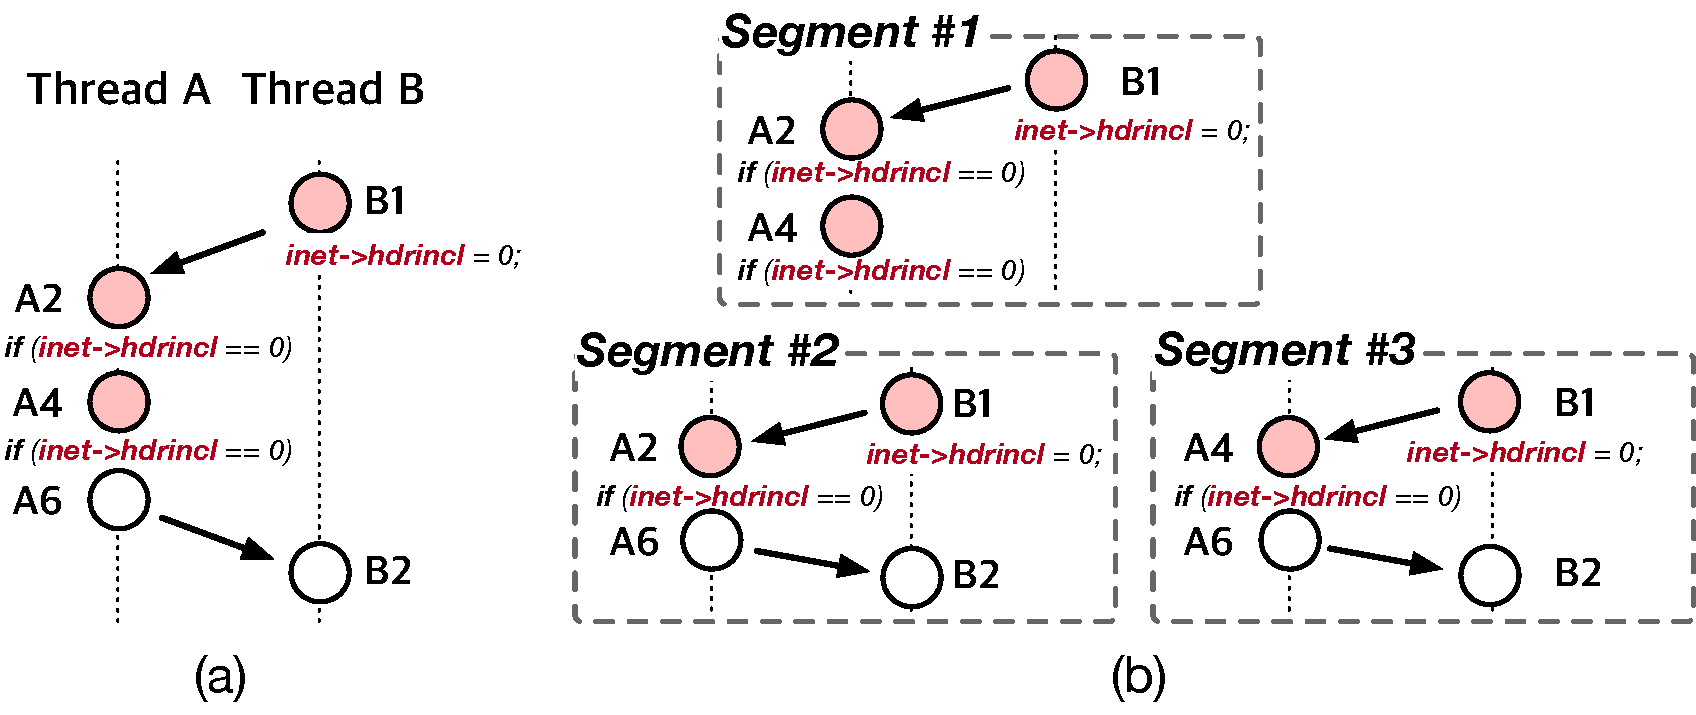
\includegraphics[width=0.9\linewidth]{fig/intuition.pdf}
  \caption{Approach overview to explore the interleaving
    space.}
  \label{fig:hint}
\end{figure}
%
\textbf{ii)} interleaving segments contained in an interleaving
instance gives promising hints for diversifying thread interleaving in
future iterations.
%
In other words, Given an interleaving segment, we can rearrange
instructions in the interleaving segment to derive \textit{unobserved}
interleaving segment.
%
\autoref{fig:hint} demonstrates how an observed interleaving segment
can be helpful for future iterations.
%
\dr{}



\subsection{Interleaving Segment Coverage}
\label{ss:coverage}

Based on the key idea, we propose a novel concurrency coverage metric
called interleaving segment coverage.
%



\newcommand{\mutable}{mutable edge\xspace}
\newcommand{\mutables}{mutable edges\xspace}
\newcommand{\immutable}{immutable edge\xspace}
\newcommand{\immutables}{immutable edges\xspace}
%
Biconflict converage is designed to track conjunctions of scheduling
constraints, and if per-input biconflict coverage is saturated, we
confidently conclude that the concurrent job unlikely causes a race
condition.

We track biconflict coverage \textit{offline}\yj{I do not get it}. During the runtime of a
kernel, the fuzzer only collects memory access operations conducted by
the concurrent job (\eg, syscalls), and after executing the concurrent
job, the fuzzer measures biconflict coverage of the concurrent job.

\PP{Definition of biconflict coverage}
%
Let us represent a memory access operation $M$ as four tuples,
$(tid, addr, op, timestamp)$ where $tid$ is the identity of a thread,
$addr$ is the address of a memory location, $op$ is the type of the
memory access operation (\ie, $store$ or $load$), and $timestamp$
indicates the point of time when the memory access operation is taken.
%
$M(x)$ detnoes a field $x$ of $M$. For example, $M(tid)$ is a $tid$
field of a memory access operation $M$.
%
Also let us suppose all memory access operations are totally
ordered. \ie, there are no two memory access operations that have the
same $timestamp$.

For all pair of memory access operations $M_i$ and $M_j$, we define a
scheduling constraint $SC$ as a tuple $(M_i, M_j)$ if
$M_i(tid) \neq M_j(tid)$, $M_i(addr) = M_j(addr)$,
$M_i(op) = store \vee M_j(op) = store$, and
$M_i(timestamp) < M_j(timestamp)$.
%
Informally, $M_i$ and $M_j$ are conflicting memory acceess operations
that are executed in other threads, and $M_i$ was taken place before
$M_j$.
%
For two scheduling constraint $SC_1(M_{1i}, M_{1j})$ and
$SC_2(M_{2i}, M_{2j})$, $SC_1 = SC_2$ if
$(M_{1i} = M_{2i}) \wedge (M_{1j} = M_{2j})$.
%
Then, we define a scheduling constraint pair $SCPair = (SC_i, SC_j)$
for two scheduling constraints if $i < j$, $SC_i \neq SC_j$.
%
Lastly, biconflict coverage of the concurrent job $BC\mbox{-}Cov$ is
defined as a set of all scheduling constraint pairs,
$\{SCPair_1, SCPair_2, ..., SCPair_n\}$, constructed from its memory
access operation sequence.



\PP{Predicting potential biconflict coverage}
%
An interleaving finding new biconflict coverage likely exposes a
behavior that was unrevealed before.
%
To discover more interesting behaviors, if new biconflict coverage is
found, the fuzzer mutates the interleaving. \ie, the fuzzer
reschedules instructions to conform with other interleavings.

Before mutating an interleaving, the fuzzer predicts \textit{potential
  biconflict coverage}, $BC\mbox{-}Cov^*$, a set of scheduling
constraint pairs that \textit{has not been observed but is expected to
  occur with other interleavings}.
%
Potential binconflict coverage will be used to direct the interleaving
mutation. \ie, the fuzzer will try to generate interleavings to expose
undisclosed scheduling constraint pairs contained in
$BC\mbox{-}Cov^*$, instead of blindly mutating an interleaving.


$BC\mbox{-}Cov^*$ is derived from biconflict coverage $BC\mbox{-}cov$,
$\{SCPair_1, SCPair_2, ..., SCPair_n\}$.
%
For each $SCPair_i$ composed of $(SC_x, SC_y)$ in $BC\mbox{-}cov$, the
fuzzer derives \dr{TODO}...



\subsection{Coverage-directed Interleaving Mutation}
\label{ss:scheduler}

\cut{
\begin{itemize}
\item an intuition for an interleaving mutation
  \begin{itemize}
  \item two observatrions
    \begin{itemize}
      \item many coverages can be executed together
      \item we can infer what coverages should be further tested
      \end{itemize}
  \item step 1: collect coverage
  \item step 2: inference of coverages to test
  \item step 3: collect coverages that can be tested together
  \item step 4: generate an interleaving to test
  \end{itemize}
\end{itemize}
}


\newcommand{\segment}{segment graph\xspace}
\newcommand{\segments}{segment graphs\xspace}
\newcommand{\Segments}{Segment graphs\xspace}


After tracking biconflict coverage of an interleaving, our
interleaving mutation takes potential biconflict coverage
$BC\mbox{-}Cov^*$ as a hint for further mutation.
%
The goal of the interleaving mutation is to generate other
interleavings that may cover scheduling constraint pairs in
$BC\mbox{-}Cov^*$.
%
Until $BC\mbox{-}Cov^*$ is not empty, the fuzzer repeats two steps of
the interleaving mutation:
%
1) selecting scheduling constraint pairs to test, and
2) generating scheduling points to test the selected scheduling
constraint pairs.

\dr{wip.}

\PP{Selecting scheduling constraints to ...}
%
Among scheduling constraint pairs in $BC\mbox{-}Cov^*$, some of them
cannot be obeyed simultaneously.
%
For example, an interleaivng obviously cannot obey the two scheduling
constraints $(X \rightarrow Y)\wedge (Z \rightarrow W)$ and
$(Y \rightarrow X)\wedge (Z \rightarrow W)$ because of the
contradiction on the execution order of $X$ and $Y$.
%
We thus 


It may require heavy computation to identify the largest subset of
$BC\mbox{-}Cov^*$ that are all harmonious to each other.
%
Instead of finding the optimal solution, we choose to use a greedy
algorithm.
%


Especially, given uncaptured \segments extracted from an interleaving
graph, our interleaving mutation starts by selecting a random
\segment.
%
And then it iteratively selects a \segment while confirming that the
selected \segment is harmonious.
%
Determining a given \segment is harmonious is conducted by checking a
loop in an accumulated interleaving graph.



\PP{Generating scheduling points}
%
After selecting harmonious \segments, generating scheduling points can
be easily done by conducting a topological
sort~\cite{topologicalsort}.
%
Since an imaginary interleaving graph is acyclic, a topological sort
always returns a sequence of vertices (\ie, instructions) that does
not violate a program order.
%
It is well known that the time complexity of a topological sort is
$O(V+E)$. Considering that the graph is sparse, $E$ is a small value
so the time complexity can be asymptotically considered as $O(V)$.
%
In this sequence, scheduling points are just instructions that the
preemption should happen; \ie, the next instruction is executed by a
different thread.
%



%%% Local Variables:
%%% mode: latex
%%% TeX-master: "p"
%%% End:
